%! TEX root = ./thesis.tex
\chapter{Einleitung}

Diese Arbeit beschäftigt sich mit algorithmischen Suchproblemen. 
Hierbei ist eine Eingabeinstanz gegeben, für welche eine entsprechende Lösung gesucht wird.
Beispiele für solche Suchprobleme sind:
\begin{enumerate}[label=\arabic*.,beginpenalty=0,midpenalty=0]
    \item Gegeben eine positive Zahl $n$, berechne die Primfaktorzerlegung von $n$.
    \item Sei $G$ eine kontextfreie Grammatik. Gegeben ein Wort $w$, berechne einen Ableitungsbaum von $w$ über $G$, oder gebe sonst „$w$ nicht von $G$ generiert“ aus.
    \item Gegeben ein Graph, berechne das größte Matching in diesem Graphen.
    \item Gegeben ein Graph, berechne eine Knotenfärbung mit drei Farben, oder gebe sonst „nicht färbbar mit drei Farben“ aus.
    \item Gegeben ein Graph, berechne eine größte Clique in diesem Graphen.
    \item Gegeben ein Graph und eine positive Zahl $k$, berechne eine Clique mit $\geq k$ Knoten in diesem Graphen, oder gebe sonst „keine Clique mit $k$ Knoten möglich“ aus.
    \item Gegeben eine aussagenlogische Formel $\phi$, bestimme eine erfüllende Belegung für $\phi$, oder gebe sonst „unerfüllbar“ aus.
    \item Gegeben eine aussagenlogische Formel $\phi$, bestimme einen Beweis (unter einem geeigneten Beweissystem, z.B. Resolution) für die Gültigkeit von $\phi$, oder gebe sonst eine Belegung an, welche $\phi$ nicht erfüllt.
    \item Gegeben einen prädikatenlogischen Satz $\phi$ in der Sprache der Arithmetik\footnote{Gemeint ist die prädikatenlogische Sprache mit einer Konstante $0$, einer unären Nachfolgerfunktion, je binären Funktionen $+$, $\times$, und binärer Relation $\leq$.}, bestimme einen Beweis (unter einem geeigneten vollständigem Kalkül, z.B. Sequenzenkalkül) für die Gültigkeit von $\phi$ ($\phi$ ist wahr in jeder Struktur), oder gebe sonst „$\phi$ ungültig“ aus.
\end{enumerate}
Innerhalb des Forschungsbereichs der theoretischen Informatik beschäftigt sich die Berechenbarkeitstheorie mit der Frage, welche dieser Aufgaben überhaupt algorithmisch berechenbar sind. Das Beispiel (9) ist z.B. überhaupt nicht berechenbar, in dem Sinn dass kein Algorithmus existiert, welcher für jeden Satz $\phi$ nach endlicher Zeit mit der korrekten Lösung antwortet.
Alle anderen Probleme (1)–(8) sind im Prinzip algorithmisch lösbar, indem alle möglichen Lösungsmöglichkeiten durchsucht werden.

Der Unterbereich der algorithmischen Komplexitätstheorie ist weniger an den prinzipiellen Grenzen von Berechenbarkeit interessiert, sondern fokussiert sich unter den berechenbaren Aufgaben damit, welche Ressourcen (Rechenzeit, Speicherplatz, zugeführte Zufälligkeit) hierfür notwendig sind. Die Komplexitätstheorie interessiert sich also dafür, welche dieser Aufgaben effizient durchgeführt werden können, und somit als umsetzbar für Computer angesehen werden. 

In der Disziplin hat sich für „Effizienz“ bzw. „Umsetzbarkeit“ insbesondere folgender Konsens durchgesetzt: ein Algorithmus ist „effizient“ wenn die Laufzeit des Algorithmus polynomiell mit der Eingabegröße wächst. Ein Algorithmus, bspw. für das Suchproblem (3), muss also der Art sein, dass eine Konstante $c>0$ existiert, sodass bei der Verarbeitung eines doppelt so großen Graphen dieser Algorithmus nur $c$-mal so lang rechnet.

\pagebreak
Unter den oben genannten Suchproblemen ist ein solcher Algorithmus mit polynomieller Laufzeit nur für Probleme (2) und (3) bekannt.
Für die Suchprobleme (1), (4), (5), (6), (7), (8) lässt sich aber ein trivialer Suchalgorithmus mit exponentieller Laufzeit angeben. Für Suchproblem (4) bedeutet das z.B., alle möglichen exponentiell vielen Zuweisungen von Farben auszuprobieren.

In der Komplexitätstheorie wurden solche \emph{Such}"-probleme wie (1)–(8) sehr früh in den Hintergrund verschoben, und stattdessen wurden die korrespondierenden \emph{Entscheidungs}"-probleme in den Blick genommen. 
Anstelle nach einer Lösung zu suchen, wird sich darauf beschränkt zu entscheiden, \emph{ob} eine Lösung existiert. Der Algorithmus muss also nur die Antwort „ja“ oder „nein“ ausgeben. Zugehörige Entscheidungsprobleme zu den oben genannten Suchproblemen wären:
\begin{enumerate}[beginpenalty=0,midpenalty=0]
    \item[2$'$.] Sei $G$ eine kontextfreie Grammatik. Gegeben ein Wort $w$, entscheide ob $w$ aus $G$ generiert werden kann.
    \item[4$'$.] Gegeben ein Graph, entscheide ob dieser Graph mit drei Farben färbbar ist.
    \item[6$'$.] Gegeben ein Graph und eine positive Zahl $k$, entscheide ob eine Clique mit $\geq k$ Knoten in diesem Graphen existiert.
    \item[7$'$.] Gegeben eine aussagenlogische Formel $\phi$, entscheide ob $\phi$ erfüllbar ist.
    \item[8$'$.] Gegeben eine aussagenlogische Formel $\phi$, entscheide ob $\phi$ gültig ist.
    \item[9$'$.] Gegeben einen prädikatenlogischen Satz $\phi$ in der Sprache der Arithmetik, entscheide ob $\phi$ gültig ist.
    \item[10$'$.] Gegeben eine Turing-Maschine $M$ und eine Eingabe $x$, entscheide ob $M$ auf Eingabe $x$ nach endlich vielen Rechenschritten terminiert.
\end{enumerate}
Beachte dass zu Suchproblemen (1), (3) und (5) keine unmittelbare Variante als Entscheidungsproblem existiert: es existiert immer eine Primfaktorzerlegung von $n$, analog existiert immer ein größtes Matching bzw. eine größte Clique in einem Graphen.
Zusätzlich führen wir auch noch das Entscheidungsproblem 10$'$ ein, für das analog keine sinnvolle Variante als Suchproblem angegeben werden kann.

Auf dem ersten Blick erscheint dieser Schwerpunkt unnatürlich. In der Praxis sind wir interessiert, effizient Lösungen zu finden, um z.B. eine Karte einzufärben (Suchproblem 4), oder um einen Sourcecode zu parsen (Suchproblem 2). Die Feststellung „Karte ist dreifärbbar“, „Sourcecode ist wohlgeformt“ der Entscheidungsalgorithmen erscheint auf dem ersten Blick wenig hilfreich.

Für diese Fokussierung auf Entscheidungsprobleme gibt es durchaus Gründe. Zum einen ist klar, dass das Suchproblem nicht einfacher sein kann, als das zugehörige Entscheidungsproblem. Die Unberechenbarkeit eines Entscheidungsproblems schließt also auch die Berechenbarkeit des Suchproblems aus. Das entspricht genau der historischen Forschungsentwicklung zum „\emph{Hilbertschen Entscheidungsproblem}“ (9$'$), worauf Turing das \emph{Halteproblem} (10$'$) reduziert hat. Mit der Unentscheidbarkeit des  Halteproblems folgt die Unentscheidbarkeit des Entscheidungsproblems (9$'$), und damit der Unentscheidbarkeit des entsprechenden Suchproblems (9). 
Das Argument lässt sich auch auf die potentiell effizient lösbaren Entscheidungsprobleme übertragen. Die Komplexitätstheorie gibt Indizien, dass die Entscheidungsprobleme (4$'$), (6$'$)–(8$'$) wahrscheinlich nicht in Polynomialzeit lösbar sind, womit unmittelbar folgt, dass auch die Suchprobleme (4)–(8) nicht in Polynomialzeit lösbar sind.

\pagebreak[3]
Für die Fokussierung auf Entscheidungsprobleme innerhalb der Komplexitätstheorie gibt es zweitens auch fachgeschichtliche Gründe: zunächst war die Trennung \emph{Entscheidungsproblem vs. Suchproblem} innerhalb der Berechenbarkeitstheorie meist nicht strikt notwendig, da „Berechenbarkeit“ zwischen den beiden Varianten meist äquivalent war. So ist die Berechenbarkeit des Hilbertschen Entscheidungsproblems (9$'$) tatsächlich äquivalent zur Berechenbarkeit des Suchproblems (9). (Falls der Entscheidungsalgorithmus „$\phi$ ist gültig“ ausgibt, dann enumeriere so lange alle Sequenzbeweise, bis einer $\phi$ beweist. Das terminiert nach Vollständigkeit des Sequenzkalküls.)
Dann stand die Komplexitätstheorie der späten 1950er Jahre nah an der Automatentheorie und der Theorie der formalen Sprachen, als diese einen ersten Vorschlag zur Unterteilung 
 der berechenbaren Aufgaben in „einfach“ und „schwer“ machten \parencite[vgl.][]{koucky_automata_2023}. Eine zentrale Unterteilung in „Schwierigkeit“ bzw. Komplexität war z.B. die Hierarchie der formalen Sprachen von Chomsky (die Regulären als sehr einfach, die Kontextfreien als etwas komplexer, die Kontextsensitiven als noch komplexer). 
Die einzig relevanten Suchprobleme – Parsing wie in (2) – haben sich dann aber auch relativ schnell geklärt (z.B. CYK-Parsing für die Kontextfreien), womit die zentralen Untersuchungsfragen wohl eher waren, welche Sprachen durch welche Grammatiken (nicht) generiert werden können, bzw. welche Automaten welche Sprachen (nicht) erkennen können. Dafür ist die Beschränkung auf die Entscheidungsvariante („Generiert die Grammatik $G$ genau die Sprache $L$? Erkennt der Kellerautomat $A$ genau die Sprache $L$?“) ausreichend zur Etablierung unterer Schranken, und ist insbesondere auch dienlich im pragmatischen Sinn. Stellvertretend sei hier \citeauthor{kozen_automata_1997} zitiert: „We do this for mathematical simplicity and because the behavior we want to study is already present at this level“ \parencite*[7]{kozen_automata_1997}.

Dieser Pragmatismus setzt sich in der ressourcenfokussierten Komplexitätstheorie fort, die seit den 1960er Jahren den Ressourcenverbrauch von Algorithmen als zentraler Indikator für „Schwierigkeit“ versteht. Das betrifft insbesondere die Klassen P und NP; hierzu lassen sich die Aufgaben (1)–(8) und (2$'$)–(8$'$) zählen.
Wieder reicht es in den meisten Fällen aus, sich auf die Entscheidungsprobleme zu beschränken.
Diese Fokussierung ist durchaus fundiert:
Einerseits, weil die zentralen algorithmischen Herausforderungen schon bei der Entscheidungsvariante auftreten („behavior we want to study is already present at this level“). So kann zum Beispiel die P-NP-Frage äquivalent als Frage über Entscheidungsprobleme auch als Frage über Suchprobleme formuliert werden. Andererseits lässt sich zeigen, dass für viele relevante Aufgaben das Suchproblem nicht schwerer ist als das Entscheidungsproblem (unter polynomieller Unschärfe). Dieses Argument wird üblicherweise als \emph{search reduces to decision} formuliert: gegeben ein effizienter Algorithmus, welcher das Entscheidungsproblem löst, kann auch ein effizienter Algorithmus angegeben werden, welcher das Suchproblem löst. Mit diesem Argument kann z.B. die Aussage „Suchproblem (7) ist effizient lösbar“ äquivalent zu „Entscheidungsproblem (7$'$) effizient lösbar“ gesetzt werden. Die Konzentration auf Entscheidungsprobleme kommt dann unter anderem auch mit dem Vorteil, dass viele theoretische Konzepte einfacher zu fassen sind und kompakter zu formulieren sind („mathematical simplicity“). Wir können uns zum Beispiel auf (laufzeitbeschränkte) Algorithmen ohne Ausgabe konzentrieren, die Eingaben nur akzeptieren und ablehnen müssen. 

\vspace{0pt plus 2ex}
\subsection*{NP-Suchprobleme als Forschungsgegenstand}

Diese Arbeit setzt genau an dieser Festhaltung an Entscheidungsproblemen an. Die zentrale Motivation dieser Arbeit besteht darin, diese identifizierte Leerstelle auf Seite der Suchprobleme zu adressieren.  Vor diesem Hintergrund wird sich diese Arbeit in vier Forschungsdesiderata den \emph{NP-Suchproblemen} im Gegensatz zu den sonst üblichen NP-Entscheidungsproblemen nähern.
Diese können als die Suchprobleme verstanden werden, die zu NP-Sprachen korrespondieren. Als Suchprobleme lässt sich eine einfache Charakterisierung formulieren: NP-Suchprobleme sind solche Suchprobleme, bei der 
\begin{itemize}
    \item die Lösung – falls sie existieren sollte – höchstens polynomiell länger als die Eingabe ist, und 
    \item effizient (d.h. in Polynomialzeit) verifiziert werden kann, ob ein fraglicher Lösungskandidat tatsächlich eine korrekte Lösung für eine Eingabe darstellt.
\end{itemize}
Das entspricht der sonst auch üblichen „Zertifikats-Definition“ der Komplexitätsklasse NP. Insbesondere induziert jede nichtdeterministische Polynomialzeit-Turing-Maschine ein NP-Suchproblem („gegeben Eingabe, finde einen akzeptierenden Rechenweg, oder gebe ‚lehnt ab‘ aus“) und umgekehrt.

Viele der anfangs genannten Suchprobleme bilden NP-Suchprobleme. Hierbei werden die „negativen Antworten“ als „es existiert keine Lösung“ verstanden. Dann ist beispielsweise das Suchproblem (4) ein NP-Suchproblem: die Färbung (Zuordnung von Knoten zu einer der drei Farben) ist höchstens so lang wie der Eingabegraph, und zu einer beliebigen Färbung (valide oder nicht) kann in Polynomialzeit überprüft werden, ob diese Färbung tatsächlich jeden zwei adjazenten Knoten eine unterschiedliche Farbe zugewiesen wird.
Die Suchprobleme (1)–(4), (6), (7) sind ebenso NP-Suchprobleme. 

Das Suchproblem (5) ist dagegen mutmaßlich kein NP-Suchproblem, denn es ist nicht bekannt wie verifiziert werden kann, dass eine Teilmenge $C$ an Knoten in einem Graph tatsächlich eine \emph{größte} Clique ist.\footnote{Suchproblem (3) fragt auch nach einer optimalen Lösung, ist aber ein pathologisches NP-Suchproblem, denn ein größtes Matching kann ohnehin in Polynomialzeit berechnet werden. Die „Verifikation“ besteht also darin zu überprüfen, ob die fragliche Lösung genau so viele Pärchen bildet wie die ad hoc berechnete optimale Lösung.}
Das Suchproblem (8) ist auch mutmaßlich kein NP-Suchproblem, denn kein Beweissystem ist bekannt, dass Gültigkeit mit polynomiell langen Beweisen ausdrücken kann. Zumindest für das Resolutionskalkül existieren spezielle gültige Formeln $\phi$ mit exponentiell langen Resolutionsbeweisen.

Die Einschränkung auf NP-Suchprobleme ist im Wesentlichen eine Konsequenz der hohen Wichtigkeit und Relevanz der Komplexitätsklasse NP, sowohl theoretisch innerhalb der Komplexitätstheorie („Wie viel hilft Nichtdeterminismus den Polynomialzeit-Berechnungen?“), als auch in der Praxis, da sehr viele interessante und in der industriellen Anwendung aufkommenden Berechnungsaufgaben als  NP-Suchprobleme formuliert werden können. Hinzu kommt die Beobachtung, dass jene Suchprobleme, welche nicht den Bedingungen von NP-Suchproblemen genügen, so gut wie definitiv zu komplex und schwer sind, um zu erwarten dass sie überhaupt effizient gelöst werden können. Für die NP-Suchprobleme (und insbesondere die nicht-vollständigen NP-Suchprobleme) ist es zumindest noch plausibel, effiziente Suchalgorithmen entwickeln zu können.

Wie aber bereits oben angesprochen, werden üblicherweise in der Literatur nicht die NP-Suchprobleme untersucht, sondern meist nur die entsprechenden NP-Entscheidungsprobleme. Das geschieht mit der Begründung, dass sich die meisten Suchprobleme auf das jeweilige Entscheidungsproblem reduzieren lassen können (\emph{search reduces to decision}). 

Als erstes Forschungsdesiderat möchte diese Arbeit genau jene Beziehung zwischen NP-Suchproblemen und NP-Entscheidungsproblemen näher untersuchen. 
Insbesondere wollen wir das \emph{search-reduces-to-decision}-Argument präzise einordnen und auch zeigen, dass dieses Argument nicht immer zutrifft, also Situationen in denen eine reine Betrachtung der Entscheidungsvarianten eigentlich nicht ausreicht. 

Tatsächlich gilt das für viele interessante Suchprobleme. Das sind zum Beispiel schon jene NP-Suchprobleme, die immer eine Lösung haben; hier kann zunächst nicht unmittelbar ein entsprechendes Entscheidungsproblem formuliert werden.
Das haben wir bereits bei den Suchproblemen (1) und (3) gesehen.
Diese \emph{totalen} NP-Suchprobleme sind insofern interessant, da viele effizient lösbar sind (z.B. Suchproblem 3), andererseits für viele die effiziente Lösbarkeit noch offen ist. Gleichzeitig wird erwartet, dass die totalen NP-Suchprobleme nicht NP-hart sind; damit ist die effiziente Lösbarkeit zumindest dieser Suchprobleme durchaus in Reichweite. 
Das trifft zum Beispiel auf das Suchproblem (1) der Faktorisierung zu. Dieses totale NP-Suchproblem ist momentan nicht effizient lösbar, aber gleichzeitig auch nicht NP-hart. Die Untersuchung solcher totalen NP-Suchprobleme geht im Wesentlichen auf \textcites{johnson_how_1988}{megiddo_total_1991} zurück.

\textcite{fenner_inverting_2003} können die Vermutung „alle totalen NP-Suchprobleme sind effizient lösbar“ in verschiedenen äquivalenten Formulierungen charakterisieren, so zum Beispiel als Invertierbarkeit von surjektiven Funktionen, oder als das effiziente Lösen des Suchproblems (7) unter Angabe einer nichtdeterministischen Turing-Maschine, welche die Menge $\mathtt{SAT}$ der erfüllbaren aussagenlogischen Formeln erkennt.
\citeauthor{fenner_inverting_2003} fassen diese jeweils äquivalenten Charakterisierungen unter der Hypothese $\hQ$ zusammen. Für diese Arbeit wird hier folgende Formulierung von  $\hQ$ angewendet, die über nichtdeterministische Turing-Maschinen spricht, welche jede Eingabe akzeptieren:
\begin{conjecture}[$\hQ$, \cite{fenner_inverting_2003}]\label{conj:q}
    Für jede nichtdeterministische Turing-Maschine $N$ mit polynomieller Laufzeitbeschränkung, und $L(N)=\Sigma^*$ existiert eine Funktion $g\in\FP$ sodass für alle $x$ das Bild $g(x)$ eine akzeptierender Rechenweg von $N(x)$ ist. 
\end{conjecture}
In dieser Formulierung wird auch die Schwierigkeit dieser Vermutung klar: wir bekommen zwar versprochen, dass $N(x)$ akzeptiert, wir wissen aber nicht, \emph{welcher} nichtdeterministische Rechenweg $x$ akzeptiert, und nicht wie wir einen solchen Rechenweg effizient berechnen könnten.

Obwohl $\hQ$ zunächst nur über totale Suchprobleme spricht, hat die Hypothese 
 $\hQ$ große Nähe und Verwandtschaft zu analogen Aussagen, die NP-Suchprobleme einerseits und die sogenannten Beweissysteme andererseits betreffen.
Als zweites Desiderat will daher diese Arbeit an den Charakterisierungen von $\hQ$ weiter arbeiten, sowie die Beziehung zwischen $\hQ$ und NP-Suchproblemen, den Beweissystemen \parencite[nach][]{cook_relative_1979} bzw. dem \emph{Pudlákschen Programm} \parencite*{pudlak_incompleteness_2017} näher untersuchen.


\subsection*{Beweissysteme und das Pudláksche Programm}

NP-Suchprobleme wie oben eingeführt korrespondieren auf natürliche Weise zu „Beweissystemen“ im intuitiven Sinn. Wir gehen das beim Suchproblem (7) durch: sollte eine Formel $\phi$ erfüllbar sein, dann existiert ein „Beweis“ für die Erfüllbarkeit von $\phi$, nämlich eben eine Belegung $w$ welche $\phi$ erfüllt. Damit ist dieses Beweissystem gewissermaßen vollständig.
Dieser Beweis ist nicht nur kurz, sondern kann effizient (gemeint ist: mit einem Algorithmus in Polynomialzeit) überprüft werden, ob der Beweis $w$ tatsächlich zu $\phi$ „passt“, also ob $w$ die Formel $\phi$ erfüllt. Damit ist dieses Beweissystem auch korrekt.

Jedes NP-Suchproblem nach der obigen Definition induziert dann ein solches korrektes und vollständiges Beweissystem. Diese Beweissysteme sind sogar insofern besonders stark, als da zu jeder korrekten Instanz ein Beweis existiert, der sogar nur polynomiell länger ist.
Insbesondere induziert ein solches Beweissystem mit polynomiell kurzen Beweisen ein NP-Suchproblem (gegeben Instanz, suche einen korrekten Beweis für die Instanz) und umgekehrt.

Das bei Suchproblem (8) angedeutete Beweissystem der Resolution für die Gültigkeit aussagenlogischer Formeln ist ein Beweissystem für die Tautologien, aber wie bereits angesprochen keins mit \emph{polynomiell langen} Beweisen. Zumindest für die Resolution bildet damit (8) kein NP-Suchproblem. 
Existiert ein polynomiell beschränktes Beweissystem für die aussagenlogischen Tautologien?

Dieser Frage gingen \textcite{cook_relative_1979} nach, und erarbeiten hierfür zunächst eine knappe und elegante Definition von aussagenlogischen Beweissystemen: \emph{Eine Polynomialzeit-berechenbare Funktion $f$ ist ein \emph{aussagenlogisches Beweissystem}, wenn der Bildbereich von $f$ mit der Menge $\mathsf{TAUT}$ der Tautologien übereinstimmt}. Wenn $f(w)=\phi$, dann wissen wir dass $\phi$ eine Tautologie ist, und dieser Fakt wird insbesondere über den Beweis $w$ im Beweissystem $f$ erfasst. 
Diese Definition erfasst damit genau die oben genannten intuitiven Eigenschaften:
\begin{itemize}[noitemsep]
    \item Die Relation \emph{„$w$ ist ein Beweis für $\phi$“} ist in Polynomialzeit entscheidbar.
    \item Das Beweissystem ist korrekt: $f$ beweist nur Tautologien.
    \item Das Beweissystem ist vollständig: zu jeder Tautologie $\phi$ existiert ein Beweis $w$, d.h. $f(w)=\phi$.
\end{itemize}
Für das Resolutionskalkül könnte ein solches aussagenlogisches Beweissystem in dieser Form so aufgeschrieben werden:
\[ h(\phi, w) \defeq \begin{cases} \phi & \text{ $w$ ist Resolutionsbeweis für die Gültigkeit von $\phi$},\\ \bot & \text{sonst}. \end{cases} \]
Hat ein aussagenlogisches Beweissystem $f$ für jede Tautologie $\phi$ einen höchstens polynomiell längeren Beweis $w$ für $\phi$, sagen wir dass $f$ \emph{kurze Beweise hat}. Das aussagenlogische Beweissystem $h$ hat \emph{keine} kurzen Beweise.
Die obere Frage, ob (8) ein NP-Suchproblem ist, lässt sich äquivalent charakterisieren mit der Frage, ob ein aussagenlogisches Beweissystem mit kurzen Beweisen existiert.
Tatsächlich beobachten \citeauthor{cook_relative_1979} sogar, dass diese Existenz äquivalent zur Aussage $\NP=\coNP$ ist.

Diese Einsicht motivierte das sogenannte \emph{Cook–Reckhow-Programm} \parencite{buss_lectures_1996}: Hierbei nähern wir uns der Frage $\NP$ vs. $\coNP$ durch Untersuchen immer stärkere aussagenlogische Beweissysteme.
Um $\NP\neq\coNP$ zu erreichen, könnten wir entweder zeigen dass kein (längen-)optimales aussagenlogisches Beweissystem (d.h. ein Beweissystem welches höchstens polynomiell längere Beweise als jedes andere Beweissystem hat) existiert, oder ein optimales aussagenlogisches Beweissystem angeben, sodass dieses keine kurzen Beweise hat.
Aufbauend auf dieser Verbindung wurden zunehmend auch untere und obere Schranken von speziellen aussagenlogischen Beweissystemen untersucht, sowie auch Beweissysteme allgemein für beliebige Mengen (und nicht nur Tautologien) betrachtet.

Die Existenz von optimalen Beweissystemen bzw. $\P$-optimalen (d.h. optimal in dem Sinn dass sogar die Beweise zwischen den Beweissystemen effizient übersetzt werden können) Beweissystemen  wurde von \textcite{krajicek_propositional_1989} in Beziehung gesetzt mit endlicher Konsistenz von mathematischen Theorien. Darauf aufbauend zeigt \textcites[Kap.~6]{pudlak_logical_2013}{pudlak_incompleteness_2017} ferner Verbindungen zwischen $\P$-optimalen bzw. optimalen Beweissystemen, Arithmetik mit exponentiell beschränkten Quantoren („\emph{bounded arithmetic}“) und der Existenz von vollständigen Elementen sogenannter \emph{Promise-Klassen}. Promise-Klassen sind solche Komplexitätsklassen, die durch speziell operierende Turing-Maschinen mit speziellen Eigenschaften erkannt werden können, wobei diese Eigenschaften üblicherweise über (Nicht)determinismus und polynomiell Laufzeit hinaus gehen. Für die Klasse $\UP\subseteq\NP$ bedeutet das z.B., dass die Sprache (wie bei NP) von einer nichtdeterministischen Polynomialzeit-Turing-Maschine erkannt werden muss, die aber – das ist der Promise – auch nur auf höchstens einem nichtdeterministischen Rechenweg akzeptieren darf.

\textcite{razborov_provably_1994} zeigt hierbei als erstes eine Verbindung zwischen der Promise-Klasse $\DisjNP$ und der Existenz von optimalen aussagenlogischen Beweissystemen. Viele weitere Beziehungen zur Existenz vollständiger Elemente der Promise-Klassen $\UP$, $ \NP\cap\coNP$, $ \DisjCoNP$ wurden ausgemacht \parencites(vgl. auch)(){messner_simulation_2001}{kobler_optimal_2003}{beyersdorff_there_2011}.
\textcite{beyersdorff_nondeterministic_2009} und \textcite{pudlak_incompleteness_2017} zeigen ferner analoge Verbindungen zu den Funktionenklassen $\NPMVt$ und $\TFNP$.

\begin{figure}[tb]
    \centering\includegraphics[page=8]{figures.pdf}
    \caption{Implikationen zwischen Pudláks Hypothesen \parencite*{pudlak_incompleteness_2017}. Beachte dass diese Implikationen relativieren.}\label{fig:pudlak-small}
\end{figure}

Motiviert durch Fragen der endlichen Widerspruchsfreiheit von Theorien und \emph{bounded arithmetic} formuliert \textcite{pudlak_incompleteness_2017} folgende Hypothesen, die hier in ihrer komplexitätstheoretischen Fassung genannt werden:\par
\medskip
\begin{tabular}{l@{\quad:\quad}l}
    $\hSAT$ & es ex. keine $\leqmp$-vollst. Menge für $\NP$ mit $\P$-opt. Beweissystem\\
    $\hTAUT$ & es ex. keine $\leqmp$-vollst. Menge für $\coNP$ mit $\P$-opt. Beweissystem\\
    $\mathsf{TAUT^N}$ & es ex. keine $\leqmp$-vollst. Menge für $\coNP$ mit opt. Beweissystem\\
    $\hNPcoNP$ & es ex. keine $\leqmp$-vollst. Menge für $\UP$\\
    $\hUP$ & es ex. keine $\leqmp$-vollst. Menge für $\NP\cap\coNP$\\
    $\hDisjNP$ & es ex. kein $\leqmpp$-vollst. disjunktes NP-Paar für $\DisjNP$\\
    $\hDisjCoNP$ & es ex. kein $\leqmpp$-vollst. disjunktes coNP-Paar für $\DisjCoNP$
\end{tabular}\par
\medskip\noindent
Seien an dieser Stelle auch schon die folgenden zwei wichtigen natürlichen Mengen definiert:
\begin{alignat*}{2}
    &\mathtt{SAT} &&\defeq \{ \phi \mid \text{$\phi$ ist eine erfüllbare aussagenlogische Formel} \},\\
    &\mathtt{TAUT} &&\defeq \{ \phi \mid \text{$\phi$ ist eine gültige aussagenlogische Formel} \}.
\end{alignat*}
Zur Notation: natürliche Mengen wie $\mathtt{TAUT}$ werden in Schreibmaschinenschrift notiert, während Hypothesen in serifenloser Schrift notiert werden.

Es muss hervorgehoben werden, dass Pudlák die Hypothese $\hTAUT$ nicht in dieser Form formuliert hat, sondern als Aussage über die Nicht-Existenz eines $\P$-optimalen Beweissystems speziell für $\mathtt{TAUT}$, genau wie anfangs des Abschnitts gefragt wurde. (In seiner Notation die Hypothese $\mathsf{CON}$.) Die beiden Charakterisierungen sind aber äquivalent; Gesagtes gilt analog auch für $\hSAT$ (vgl. Abschnitt~\ref{sec:prelim-ps}).


Insbesondere arbeitet Pudlák die Beziehung zwischen diesen einzelnen Hypothesen heraus, und kommt hierbei zu Abbildung~\ref{fig:pudlak-small}, die anzeigt, wie die bekannten Implikationen zwischen den oberen Hypothesen verlaufen.
Auf der Seite der Komplexitätstheorie fragt Pudlák im Speziellen nach natürlichen plausiblen stärkeren Hypothesen (die z.B. sowohl $\hTAUT$ als auch $\hTFNP$ implizieren, wobei Pudlák diese beiden Hypothesen jeweils als plausibel ansieht), sowie im Allgemeinen nach Separationen zwischen diesen Hypothesen. Zum Beispiel kann durch Angabe von Orakeln gezeigt werden, dass zwei Hypothesen unter relativierbaren Beweisen nicht gleich sind, oder stärker sogar unabhängig unter relativierbaren Beweisen sind. 
%Das wird später näher erläutert.
Dieses allgemeine Forschungsdesiderat fasse ich für diese Arbeit lose als \emph{Pudláksches Programm} zusammen.

Die vorliegende Arbeit will drittens an genau diesem Pudlákschen Programm beitragen, indem im Wesentlichen die Übersicht in Abbildung~\ref{fig:pudlak-small} verfeinert wird, und dabei stärkere (und schwächere) Hypothesen eingeordnet werden. Hierbei fokussiere ich mich insbesondere auf jene Hypothesen, die mit NP-Suchproblemen im Zusammenhang stehen, wie z.B. $\hQ$.
Im Folgenden sei noch auf den „Orakel“-Teil des Pudlákschen Programms eingegangen.


\subsection*{Orakel und Relativierungen}

Orakel und Orakel-Turing-Maschinen sind ein Begriff aus der Berechenbarkeitstheorie um die relative Schwierigkeit von algorithmischen Entscheidungsproblemen zu untersuchen, die über \emph{berechenbar vs. unberechenbar} hinaus gehen. Wenn eine Turing-Maschine eine Abstraktion eines Computers darstellt, dann ist ein Orakel eine Abstraktion einer Datenbank in der Cloud, die vom Computer angerufen werden kann, um zu fragen, ob ein gewisser Eintrag in der Datenbank liegt. Dieses Abfragen des Entscheidungsproblems („Ist Eintrag in Datenbank?“) kann der Computer gewissermaßen gratis durchführen.

Formal werden Orakel als Mengen $A$ realisiert, und Orakel-Turing-Maschinen dürfen für beliebige aufgeschriebene Wörter $w$ abfragen, ob $w\in A$ liegt. Ist nun $A$ insbesondere eine unberechenbare Menge, dann kann die zugehörige Turing-Maschine auch komplexere Mengen entscheiden, die sonst unberechenbar wären.
\textcite{post_recursively_1944} arbeitet aus diesem Begriff die Turing-Reduzierbarkeit aus: $A$ ist auf $B$ Turing-reduzierbar wenn $A$ über eine Orakel-Turing-Maschine mit Orakel $B$ entschieden werden kann. In anderen Worten: $A$ kann mittels Hilfe von Orakel $B$ entschieden werden.  Damit können sonst unberechenbare Mengen $A$ und $B$ nach ihrer relativen Schwierigkeit \emph{über einfache Berechenbarkeit hinaus} geordnet werden können. Diese Ordnung ermöglicht zum Beispiel die Unterteilung der unentscheidbaren Mengen in \emph{Grade der Unlösbarkeit}.

\textcite{cook_complexity_1971} überträgt diese Form von Reduzierbarkeit auf den polynomiellen Bereich der Komplexitätstheorie, um so die relative Komplexität zwischen zwei Mengen $A$ und $B$ unter polynomieller Unschärfe einzuschätzen: $A$ ist auf $B$ Cook-reduzierbar wenn $A$ mit einer Orakel-Turing-Maschine mit Orakel $B$ in Polynomialzeit entschieden werden kann. Auf ähnliche Weise wurde der Begriff von Orakeln im polynomiellen Bereich eingesetzt, um die Polynomialzeit-Hierarchie zu definieren, womit NP generalisiert wird, und der Komplexitätsraum zwischen P und PSPACE verfeinert werden kann.

Neben diesen deskriptiven Eigenschaften haben sich Orakel als nützliches beweistheoretisches Werkzeug in der Komplexitätstheorie erwiesen. Die zentrale Einsicht hierbei ist, dass viele der „üblichen“ mathematischen Beweismethoden, welche in der Komplexitätstheorie eingesetzt werden, \emph{relativieren}. Das bedeutet, dass diese mathematischen Beweise nicht nur die eigentliche Aussage (wie z.B. der Hierarchiesatz $\P\neq \mathrm{E}$) beweisen, sondern für jedes Orakel $A$ diese Beweise auch die \emph{relativierte} Aussage beweisen, bei der  alle beteiligten Turing-Maschinen Zugriff auf das Orakel $A$ bekommen. Die Aussage $\P\neq \mathrm{E}$ relativiert so zur Aussage $\P^A\neq \mathrm{E}^A$ für jedes $A$, das bedeutet dass eine Menge $L$ existiert, die von einer Exponentialzeit-Orakel-Turing-Maschine mit Zugriff auf $A$ erkannt wird, aber keine Polynomialzeit-Turing-Maschine (selbst mit Orakel-Zugriff auf $A$) kann $L$ entscheiden.

Damit werden speziell konstruierte Orakel zu einem Indiz, dass gewisse Aussagen schwer zu beweisen sind.
Beispielsweise konstruieren \textcite{baker_relativizations_1975} ein Orakel $A$ sodass $\P^A\neq \NP^A$. Mit diesem Fakt ist die Aussage „$\P=\NP$“ nicht mit relativierbaren Methoden beweisbar, da sonst ja auch $\P^A=\NP^A$ gelten würde. Tatsächlich zeigen \citeauthor{baker_relativizations_1975} sogar zusätzlich, dass $\P^B= \NP^B$ für ein zweites Orakel $B$. Damit kann also auch die Aussage „$\P\neq\NP$“ nicht mit relativierbaren Methoden bewiesen werden. Nimmt man diese beiden Indizien zusammen, ergibt sich dass die P-NP-Frage \emph{unabhängig} unter relativierbaren Beweisen ist.

Im Kontext des Pudlákschen Programms wurde für viele potentielle Implikationen (wie z.B. $\hDisjCoNP\Rightarrow\hTAUT$) ein Orakel konstruiert, relativ zu diesem diese Implikationen nicht gelten (es existiert ein Orakel, relativ zu dem $\hDisjCoNP$ gilt aber nicht $\hTAUT$). Entsprechende Konstruktionen wurden unter anderem von \textcites{glaser_disjoint_2004}{dose_np-completeness_2019}{dose_balance_2020}{dose_further_2020}{dingel_separation_2022}{ehrmanntraut_oracle_2022}{khaniki_new_2022} entwickelt. Damit wird plausibilisiert, dass gewisse Hypothesen des Pudlákschen Programms tatsächlich unterschiedlich sind.

Diese Arbeit reiht sich in dieses Arbeitsvorhaben direkt ein, und wird viertens ein weiteres Orakel konstruieren, um Hypothesen (unter relativierbaren Beweisen) zu trennen.

\subsection*{Beitrag und Überblick}

Der Aufbau der Arbeit und die einzelnen Beiträge sind hier noch einmal zusammengefasst.

Im nächsten Kapitel~\ref{chap:prelim} klären wir die notwendigen mathematischen Grundlagen. Insbesondere definieren wir präzise den Begriff des (Cook–Reckhow-)Beweissystems und den der Relativierungen, welche bereits oben angesprochen wurden.

Im Kapitel~\ref{chap:searchproblems} formalisieren wir den oben bereits intuitiv erfassten Begriff der NP-Suchprobleme und totalen NP-Suchprobleme. 
Wir werden diese außerdem mit Funktionenklassen gegenüberstellen und einen Reduktions- und Vollständigkeitsbegriff über die sogenannte Levin-Reduzierbarkeit auf NP-Suchproblemen definieren.

Der Rest dieses Kapitels hat dabei den Charakter eines Überblickswerks bzw. eines Surveys. 
Einerseits wird die Beziehung zwischen NP-Suchproblemen und NP-Entscheidungsproblemen erläutert, was auch das \emph{search-reduces-to-decision}-Argument umfasst. Es werden Ergebnisse zusammengetragen, wann dieses Argument zutrifft, und wann es insbesondere nicht zutrifft.
Andererseits werden Arbeiten vorgestellt und eingeordnet, welche gemeinsame Eigenschaften und Strukturen von NP-Suchproblemen untersuchen. Besonders interessant sind hierbei die vollständigen NP-Suchprobleme, die sich ähnlich zu den sonst üblichen NP-vollständigen Mengen/Entscheidungsproblemen verhalten. Hierbei lässt sich – analog zur Berman–Hartmanis-Isomorphievermutung – zu vielen NP-vollständigen Suchproblemen eine gemeinsame Struktur bzw. Isomorphie erkennen.

In Kapitel~\ref{chap:pudlak} werden wir Hypothesen zu NP-Suchproblemen und die Aussage $\hQ$ in das Pudláksche Programm einordnen. Erstens untersuchen wir, ob die (Levin-)Vollständigkeit eines NP-Suchproblems  mit der (Karp-)Vollständigkeit des entsprechenden NP-Entscheidungsproblems übereinstimmt. Insbesondere wird plausibilisiert, dass diese Übereinstimmung nicht gilt.
Zweitens werden wir (nicht-relativierbare) Charakterisierungen von $\hQ$ durch \textcite{fenner_inverting_2003} und \textcite{kobler_is_2000} verallgemeinern und relativieren, womit wir als Nebeneffekt auch präzise zu (relativierbaren) Implikationen zwischen $\hQ$ und den Pudlákschen Hypothesen kommen.
Drittens wird zum Abschluss des Kapitels, wieder in Form eines Surveys, das Pudláksche Programm durch das Hinzufügen weiterer Hypothesen erweitert und verfeinert, welche in der Literatur diskutiert werden.
Hinzu erarbeiten wir eine Übersicht über die Implikationen zwischen diesen Hypothesen, sowie Orakeln welche diese Implikationen unter relativierbaren Beweisen trennen. Im Wesentlichen wird Abbildung~\ref{fig:pudlak-small} zu Abbildung~\ref{fig:figure-implications} und~\ref{fig:oracles} (S.~\pageref{fig:figure-implications}, \pageref{fig:oracles}) vergrößert.

Im Sinne dieser Trennung unter relativierbaren Beweisen wird in Kapitel~\ref{chap:orakel} ein Orakel konstruiert, relativ zu diesem $\hDisjNP$ und $\hUP$ und $\hQ$ gilt. Damit gibt es also keinen relativierbaren Beweis für $\neg\hQ$, selbst wenn man beide Pudlákschen Hypothesen $\hDisjNP$ und $\hUP$ annimmt. Insbesondere wird damit der erste Schritt unternommen, die relative Stärke der Hypothese $\hQ$ gegenüber den anderen der Pudlákschen Hypothesen unter relativierbaren Beweismethoden abzugrenzen. 

Die Arbeit endet mit einer abschließenden Diskussion in Kapitel~\ref{chap:conclusion}, erläutert die Ergebnisse noch einmal, und trägt die offenen Fragen zusammen, welche in den vorigen Kapiteln gestellt wurden.




